% Chapter Template

\label{chpt:observations and observational techniques} % for referencing this chapter elsewhere, use \ref{chpt:label}
\lhead{\emph{Observations, and observational techniques}} % This is for the header on each page - perhaps a shortened title

In CVs with a sufficiently high inclination ($\gtrsim 80 \deg$, depending on mass ratio) the donor star will eclipse the white dwarf, accretion disc, and bright spot of the system in quick succession once per orbit. Observing and modelling these eclipses, with knowledge of the orbital period and the temperature of the white dwarf, can yield a thorough characterisation of the CV. The methodology for this characterisation is described in detail in \S\ref{chpt:modelling and techniques}, but essentially relies on extracting the white dwarf temperature, mass, and radius from the white dwarf colours and system parallax, then combining the white dwarf mass and radius with the timing of various eclipse features to find the key parameters of donor mass, donor radius, and orbital separation. In other words, to properly characterise a CV we need flux-calibrated, high time resolution, multi-colour photometery of the target.

The work of this thesis has made extensive use of three instruments: ULTRASPEC, ULTRACAM, and HiPERCAM.
These are time-series photometric imaging cameras, capable of taking high-cadence images of the night sky in one, three, or five colours, respectively.
The eclipses we observe typically span around 30 minutes and need to measure flux changes on timescales of a few seconds to be useful for analysis.
Crucially, HiPERCAM and ULTRACAM make their multi-colour images simultaneously, which removes the possibility of changes in brightness in the disc or bright spot polluting the white dwarf colour measurement, making them ideal instruments for this analysis.


\section{Instruments}
\label{sect:observations:cameras}

The cameras used were mounted on several telescopes across the decade of our observations. These were the Gran Telescopio de Canarias (GTC) on La Palma (with HiPERCAM), the Thai National Telescope (TNT) with ULTRASPEC, the New Technology Telescope (NTT) in Chil\'e (with ULTRACAM). Prior to [YEAR]\todo{When was ULTRACAM taken off the WHT? 2014, I think?}, ULTRACAM was hosted on the William Herschel Telescope (WHT), also on La Palma. Table~\todo{Table of observations} details what instrument/telescope combination was used for each observation used in this thesis.


\subsection{HiPERCAM}
\label{sect:observations:hipercam}

HiPERCAM is a quintuple-beam optical imaging camera, that saw first light on the GTC in 2018 and is sensitive to wavelengths from $320 - 1060 \rm nm$ \citep{dhillon2021}.
HiPERCAM uses a system of Super SDSS filters ($u_{\rm sup}, g_{\rm sup}, r_{\rm sup}, i_{\rm sup}, z_{\rm sup}$), designed to match the classic SDSS band cutoff wavelengths \citep{fukugita1996}, but allow a higher throughput and so give a more sensitive instrument.
This camera has a series of dichroic beamsplitters, that sequentially pick off the $u_{\rm sup}, g_{\rm sup}, r_{\rm sup}, i_{\rm sup}, z_{\rm sup}$ bands and funnel each into dedicated cameras that use highly sensitive, low readout noise electron-multiplying Charge-Coupled Devices (CCDs).
However, this improvement is not constant across the bands, shown in Figure~\ref{fig:observations:superSDSS throughput comparison}, resulting in a small difference between colours observed with HiPERCAM and SDSS.
Unfortunately, as our calibrating standard stars are reported in the classic SDSS photometric system, some work was necessary to color-correct the HiPERCAM observations, which is described in detail in \S\ref{sect:observations:colour correction method}.
\begin{figure}
    \centering
    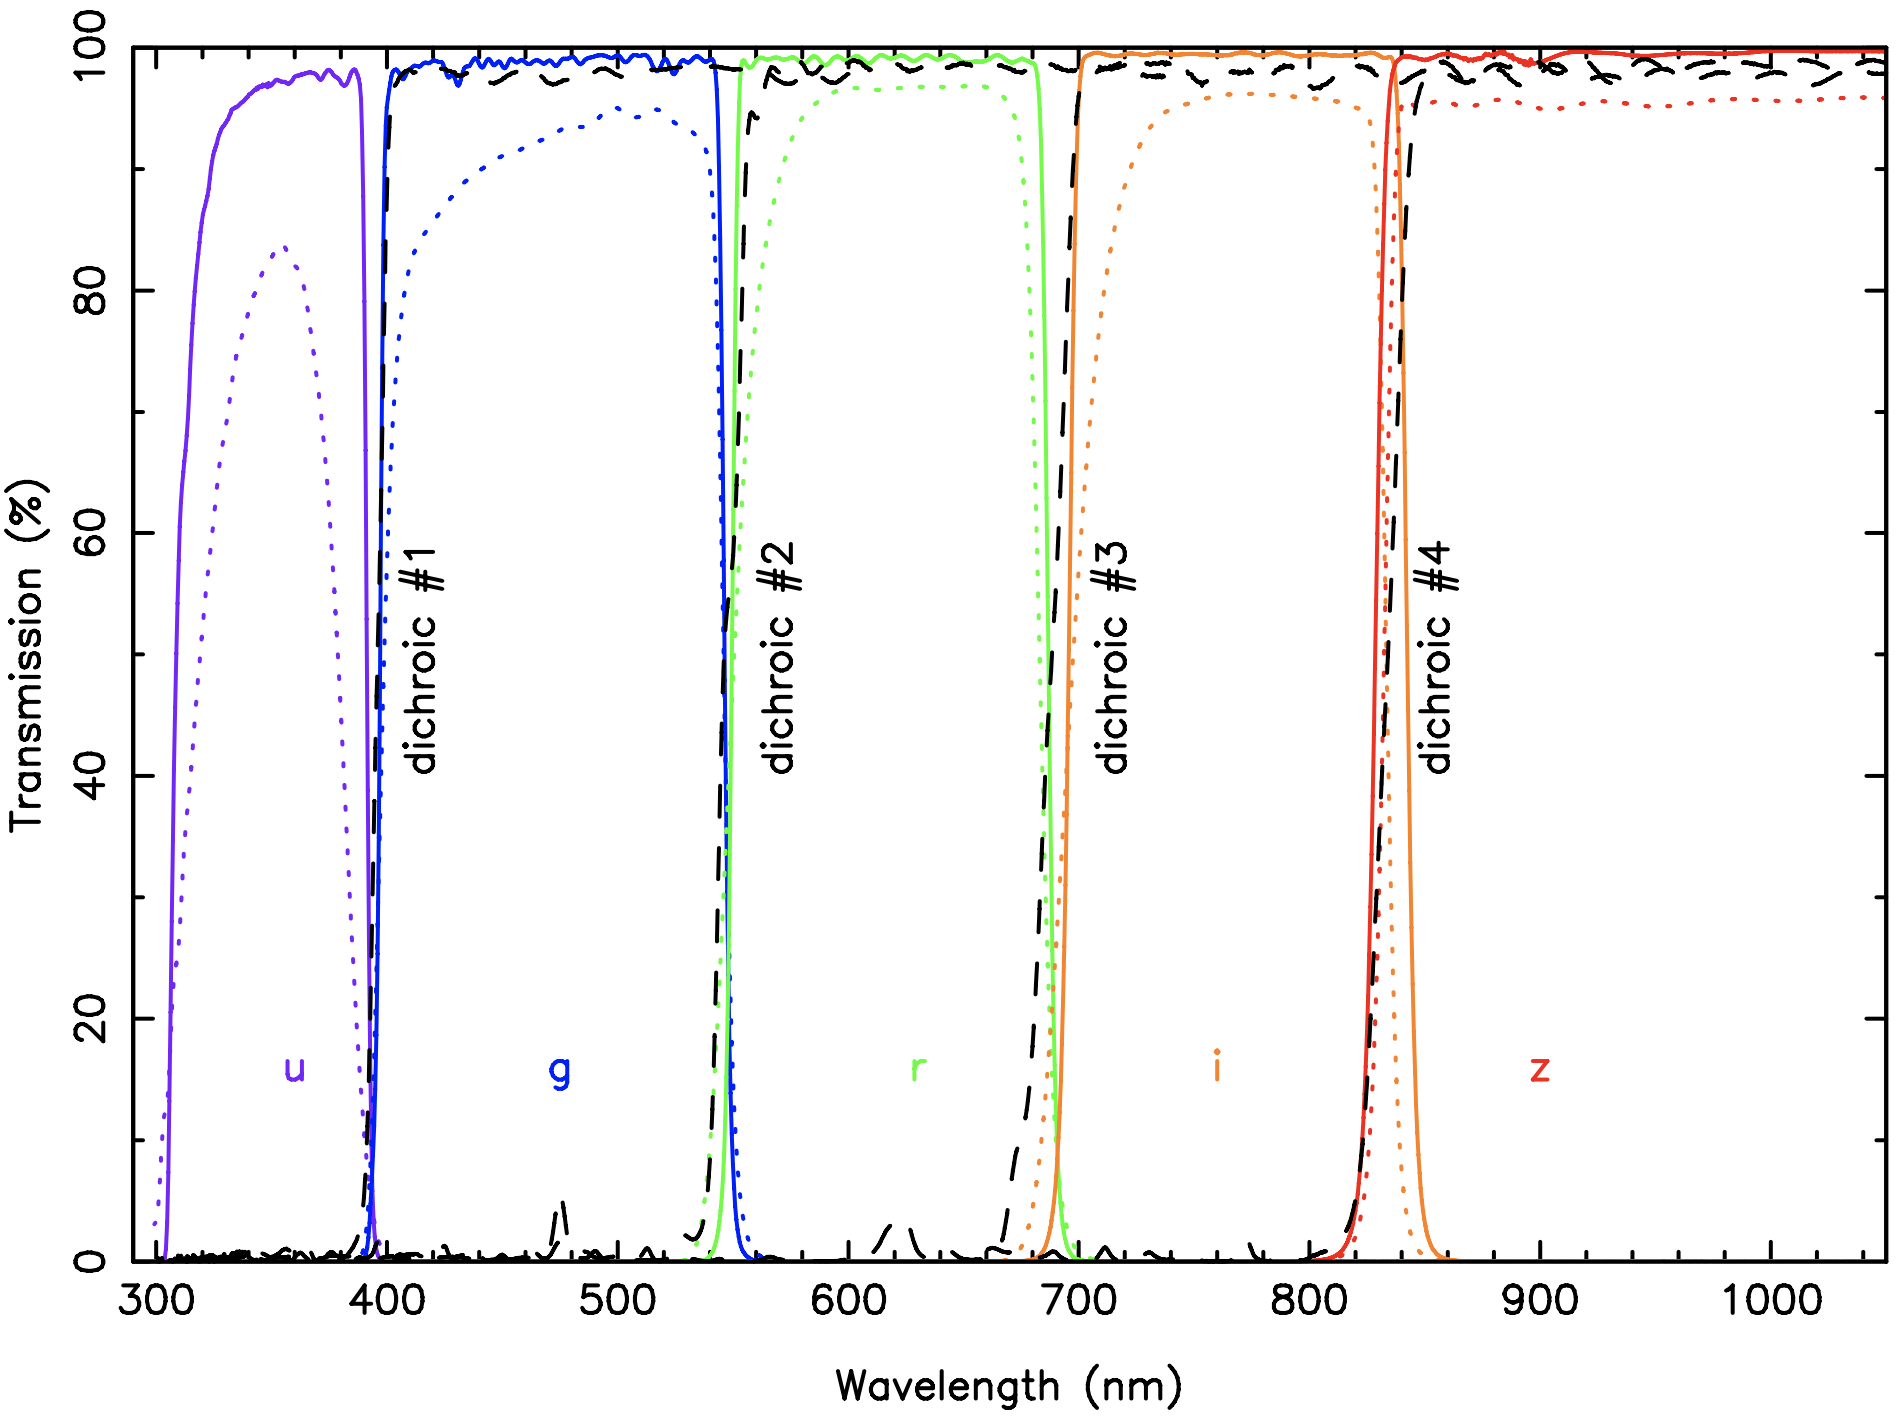
\includegraphics[width=0.7\textwidth]{figures/observations/plot_dichs_supersdss_asbuilt_v3.png}
    \caption{Taken from \citet{dhillon2021}. Transmission profiles of the as-built HiPERCAM dichroic beamsplitters ({\bf dashed black lines}), the HiPERCAM standard SDSS filters ({\bf dotted lines}), and the HiPERCAM Super SDSS filters ({\bf solid lines}).}
    \label{fig:observations:superSDSS throughput comparison}
\end{figure}

On the GTC, HiPERCAM is capable of detecting sources down to $g_{\rm sup} \sim 23$ in exposures of only a second, and can achieve $g_{\rm sup} \sim 28$ with an hour of exposure. This has allowed us to make excellent observations of fainter CVs than previous studies (e.g. \citealt{McallisterThesis}), and helps target CVs at short periods with faint, low mass donors.

HiPERCAM is capable of incredibly fast framerates of up to $\sim 1000 \rm Hz$, though this capability was not used for this work.
However, as part of the effort to achieve this framerate by reducing dead-time between frames HiPERCAM is capable of exposing a frame while {\it simultaneously} reading out the previous image.
This is achieved by splitting the photodetector in half, and masking one side. When a frame is finished exposing, it is shuttled across to the masked side (a rapid process, $6.8 - 7.8$ms) and can be read out during the next exposure time. To compensate up for masking half of a CCD, two CCDs side-by-side are used to emulate a single full-frame detector.
This virtual elimination of dead-time is a significant benefit when resolving the large, rapid changes in flux during the ingresses and egresses of CV eclipses.


\subsection{ULTRACAM}
\label{sect:observations:ultracam}

ULTRACAM is a three-beam optical imager sensitive to wavelengths between $\sim 300 - 1100 \rm nm$, and is the direct predecessor to HiPERCAM \citep{dhillon2007}.
It is similarly built for high-speed photometric studies, but is not capable of the extreme framerates of HiPERCAM, limited to framerates of $\lesssim 500 \rm Hz$.
ULTRACAM uses the same split-frame readout technique to HiPERCAM, though uses more typical CCDs rather than HiPERCAM's electron-multiplying CCDs.

ULTRACAM was originally commissioned with SDSS-like $u',g',r',i',z'$ filters, that match the SDSS closely and did not necessitate colour-term corrections. However, in [YEAR] \todo{When did we move to super SDSS on ultracam? 2018?} ULTRACAM was upgraded to use the same Super SDSS photometric system used by HiPERCAM. When necessary, observations were translated to the classic SDSS system as described in \S\ref{sect:observations:colour correction method}.
Observing an object with ULTRACAM in more than three bands requires multiple observing runs, and manually swapping filters.


\subsection{ULTRASPEC}
\label{sect:observations:ultraspec}

Finally, the ULTRASPEC camera was occasionally used to supplement ULTRACAM and HiPERCAM observations. ULTRASPEC was originally commissioned as a spectrographic cousin of ULTRACAM, using again a split-frame design, with electron-multiplying CCDs \citep{dhillon2014}.
After a brief proof-of-concept trial as a photometric imager in June 2009, ULTRASPEC was modified to a full-time imaging instrument and mounted on the 2.4m TNT in November 2013, and is now operated by the National Astronomical Research Institute of Thailand (NARIT).

This is a single-colour instrument that uses the $u',g',r',i',z'$ filters, in addition to a wide-band KG5 filter that is approximately equivalent to $u' + g' + r'$. It is also the slowest of the three cameras, but is still capable of high framerates up to $\sim 200 \rm Hz$. However, as ULTRASPEC on the NTT is a somewhat less powerful instrument than either HiPERCAM or ULTRACAM, it proved useful in two significant respects - to gauge the viability of CV systems before dedicating more valuable HiPERCAM and ULTRACAM observing time (e.g. testing the visibility of eclipse features, checking if a CV is undergoing an outburst), and in acquiring or refining measurements of orbital period.


\section{Data reduction}
\label{sect:observations:data reduction}

All three cameras use CCD detectors, which are a staple of ground-based astronomy due to their high sensitivity, and low noise.
CCDs are made up of a large grid of photosensitive pixels, which release electrons proportionally to the number of photons that fall on them. This signal is then moved pixel-by-pixel into the readout electronics, which is essentially a capacitor that has its voltage measured to determine the number of electrons that were released. This voltage is converted to electron counts with an Analog-to-Digital Converter (ADC), that outputs the corresponding integer number of electrons to the input charge, in Analog-to-Digital Units (ADU).

To extract time-series photometric information from the raw image files, the HiPERCAM data reduction pipeline was used\footnote{Available https://cygnus.astro.warwick.ac.uk/phsaap/hipercam/docs/html/}.
\todo{Is this ok?}The analysis of this data was done with flux-calibrated relative photometry, in which a reference star in the same image as the target is extracted and used as a known-constant flux source. Then, by using the ADU flux ratio between these two sources as the observable, effects from changes in weather, altitude, and seeing conditions are removed, since these variations affect both the target and reference star equally. By multiplying the ADU flux ratio between the target and reference stars by the flux in mJy of the reference star, we can calibrate our photometry and produce a lightcurve of the target star, in units of energy flux.
% Bias and flat field corrections are done for each observation, with calibration frames taken nightly as standard procedure.


\subsubsection{Bias frames}
\label{sect:observations:bias frames}

\begin{figure}
    \centering
    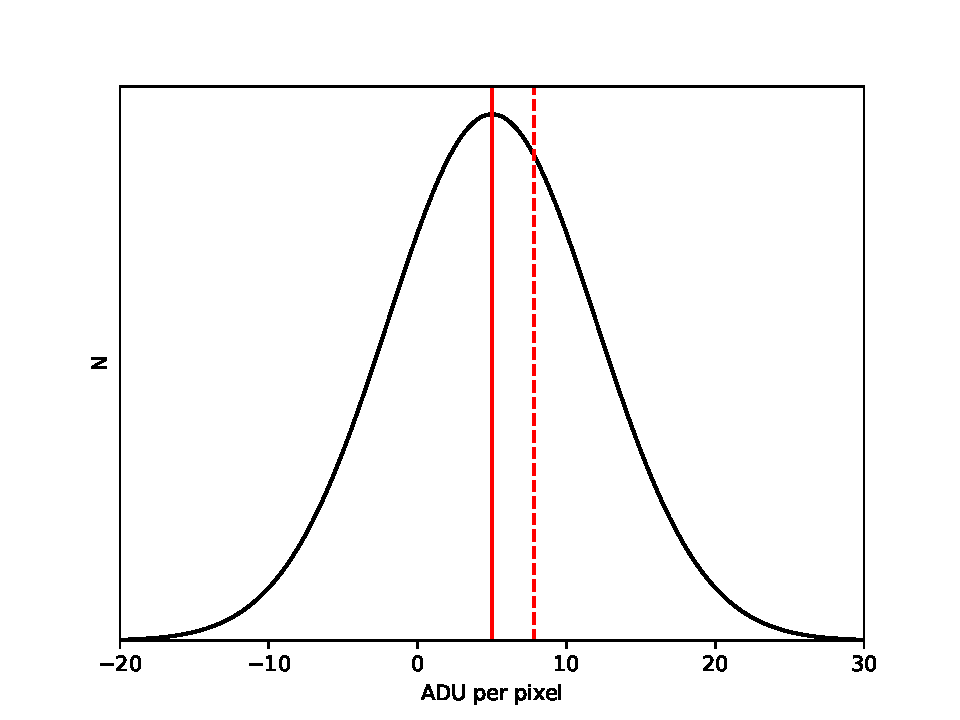
\includegraphics[width=0.7\textwidth]{figures/observations/bias_frame_histogram.pdf}
    \caption{Illustrating the effect of omitting negative values on the average of a distribution. The {\bf black line} is a Gaussian distribution with an average of 5 and a standard deviation of 7. The {\bf vertical dashed line} shows the `true' average of 5 ADU, and the {\bf vertical solid line} shows the average given by an ADC that reports negative electron counts as 0.}
    \label{fig:observations:bias frame histogram}
\end{figure}
The readout electronics of a CCD are not perfect, and contribute a small amount of gaussian noise to each pixel called readout noise. The ADC is only capable of recording {\it positive integer values}, and rounds negative pixel counts to 0. To illustrate why this is an issue, take the exaggerated example of a readout noise of $7 e^-/{\rm px}$ on a region of the CCD that is stimulated by $5 e^-/{\rm px}$. If negative values are limited to 0, the effect is to increase the average, and Figure~\ref{fig:observations:bias frame histogram} illustrates the effect of discarding negative counts.
This will have a small corrupting effect on low-signal areas of the CCD, namely the sky background signal that needs to be subtracted from the source signal (\S\ref{sect:observations:aperture photometry}).

To prevent corruption, a small bias voltage is applied to each pixel, raising the null detection value away from zero and preventing noise from giving negative readings.
To then remove this bias voltage from observations, zero second exposures of a masked detector are taken to characterise the bias voltage for each pixel, and are subtracted off each subsequent exposure. These are known as bias frames, and because the structure of the bias is subtly altered by different instrument setups, a new bias frame is taken when instrument options such as binning pixels together when reading them out, or only reading out partial images, are altered.


\subsubsection{Flat fielding}
\label{sect:observations:flat field frames}

The response of each pixel to photons is similar, but not exactly equal. In addition, the optics of the telescope are not perfect and throughput varies across the field of view, a.k.a vignetting Dust and imperfections in the telescope optics can also introduce variation across the image. Finally, as filters cannot be manufactured with perfect uniformity, each filter also makes a contribution to variations across an image\todo{Not 100\% sure on that last one...}.
These effects mean that each exposure the instrument takes is convolved with a constant flat-field response pattern.

In order to characterise and remove the flat-field pattern, an exposure is taken of an image that is known to be uniform in brightness, for example a specialised light box with a high degree of uniformity, which will have the flat-field pattern imprinted on it.
A simpler approach to a specialised light box is to observe the sky during sunset, when the sky is still bright and the contribution of light from stars is negligible. In the absence of cloud, the twilight sky forms a highly uniform field in optical bands.
Residual stellar light should still be removed though, so to completely eliminate stars from the flat field observation many exposures are taken while the telescope is being nudged by a small amount every few seconds. Since the stars move between each exposure, calculating the median frame will remove stars from the image, leaving behind only the uniform sky observation imprinted with the flat-field response pattern.
The flat field images are bias corrected to give the final flat image.
Then, by dividing each subsequent exposure by the flat image, we can correct for non-uniformity in the detector response in future images.


\subsubsection{Aperture photometry}
\label{sect:observations:aperture photometry}

While stars are theoretically point sources we observe them through the atmosphere and the optics of the telescope, which act to spread the light from a star by typically a few arcseconds even under the best conditions - spreading light from a star over several pixels. As such, to find the total flux of a star we must sum the contributions from all pixels containing the stars' flux, and the HiPERCAM pipeline has two methods for this: `normal' extraction and `optimal' extraction.

The sky background is not perfectly black and in both extraction methods must be removed from the extracted flux of a source. This is done by taking an annulus about each source, and assuming it is solely make up of sky background light (in the case of a nearby object, it can be masked in software and not counted in the sky background). The inner edge of the annulus is selected to be far enough from the source that none of the target's light is present, and the outer edge is limited by large annuli starting to become sensitive to sky variations across the image. The average sky signal per pixel is then calculated, and subtracted to isolate the source flux.

Under normal extraction, the user specifies one or more `reference' stars, and one or more `target' stars. The pixel ADU counts around the reference stars as a function of their radial distance to the peak flux are characterised with a Gaussian or Moffat profile. The Full-Width at Half Maximum (FWHM) of this distribution fit is calculated, and all pixels within $x \times \mathrm{FWHM}$ of the peak flux are summed to give the extracted flux of a source, cutting off some amount of the wings of the flux distribution. Here $x$ is a user-defined parameter, and while in theory a large value of $x$ would be desirable to capture all flux from a source, adding extra pixels increases the readout noise of the detection, and suffers from diminishing returns due to the small amounts of flux contained in the wings.
Also, as the same fraction of light from each source should be lost from both the target sources and reference sources, cutting out these wings should not alter the flux ratio between sources, and the flux ratio is the relevant quantity under relative photometry (see \S\ref{sect:observations:photometric extraction and calibration}).

In many cases, it is preferable to use the `optimal' extraction method, described by \citet{naylor1998}. Here, a weight is taken into account when summing the flux contributions of each pixel based on the {\it expected} contribution to the overall flux. This can give an improvement of $\sim 10\%$ to the signal-to-noise ratio, especially in faint sources as this approach is more robust against poor profile fits. Source profiles can diverge from the idealised Gaussian or Moffat profiles due to noise or inconsistencies in seeing conditions, and these effects are more pronounced in fainter sources.



\section{Photometric calibration}
\label{sect:observations:photometric extraction and calibration}

A comparison star in the same frame as the target is used to account for seeing and transparency variations over an observation, and standard stars from \citet{smith2002} were used to transform the lightcurves from ADU to the SDSS $u'g'r'i'z'$ photometric system. At the core of the photometric calibrations is the following expression of the apparent magnitude in some band, $m_{app}$, of a target,
\begin{equation}
    \label{eqn:observations:instrumental magnitude from scratch}
    m_{app} = m_{inst} + \chi k_{ext} + m_{zp} + C_{inst}c_{m}
\end{equation}
where $m_{inst}$ is the instrumental magnitude, $-2.5 \rm log(ADU flux)$, $\chi$ is the airmass of the observation and $k_{ext}$ is the atmospheric extinction coefficient in the relevant band. $m_{zp}$ is the zero point offset of the instrument, calculated from photometric standard stars, ideally taken on the night of an observation. $c_{m}$ is the colour term correction between the response curve of the instrument, and the target photometric system, and $C_{inst}$ is a diagnostic instrumental colour. Each of these terms must be properly handled, and are discussed in turn.


\subsection{Calculating atmospheric extinction coefficients}
\label{sect:calcualting atmospheric extinction}

Atmospheric extinction was calculated using the longest continuous observation available within a reasonable time from target observations.
The atmospheric extinction values are reported in Table~\ref{table:atmos_extinction}\todo{Currently, this is only for a very narrow range of the actual observations. Generalise this table to include all instruments and locations.}.

To calculate the atmospheric extinction coefficients, aperture photometery was extracted for five sources in these long observations, and the instrumental magnitude, $m_{\rm inst}$, vs airmass, $\chi$, was fit with a straight line for each source.
The gradients of these lines are the atmospheric extinction coefficients, $k_{\rm ext}$, for the relevant band, and the y-intercept is the instrumental magnitude of that object above the atmosphere, $m_{\rm inst,0}$:
\begin{align*}
    m_{\rm inst} =& m_{\rm inst,0} + \chi k_{\rm ext}
\end{align*}

\begin{table}
    \centering
    \caption{Typical atmospheric extinction coefficients for La Silla, derived from ULTRACAM/NTT observations.}
    \label{table:atmos_extinction}
    \begin{tabular}{cccc}
        \hline
        Date of Observation & Airmass Range & Band & $k_{ext}$ \\
        \hline
        \hline
        14 Oct 2018   & 1.30-1.98 & $u_{\rm reg}$ & $0.4476$ \\
                      &           & $g_{\rm reg}$ & $0.1776$ \\
                      &           & $r_{\rm reg}$ & $0.0861$ \\
        \hline
        30 Sept 2019  & 1.03-1.63 & $u_{\rm sup}$ & $0.4867$ \\
                      &           & $g_{\rm sup}$ & $0.1803$ \\
                      &           & $r_{\rm sup}$ & $0.0713$ \\
        \hline
    \end{tabular}
\end{table}


\subsection{Transformations between filter systems}
\label{sect:observations:colour correction method}

ULTRACAM and HiPERCAM use an SDSS-\emph{like} filter system with higher efficiency bandpasses, referred to as Super SDSS. There are three relevant photometric paths:
\begin{itemize}
\item SDSS filters, $u', g', r', i', z'$;
\item ULTRACAM/ULTRASPEC SDSS-like, $u_{\rm reg}, g_{\rm reg}, r_{\rm reg}, i_{\rm reg}, z_{\rm reg}$;
\item HiPERCAM/ULTRACAM Super SDSS, $u_{\rm sup}, g_{\rm sup}, r_{\rm sup}, i_{\rm sup}, z_{\rm sup}$.
\end{itemize}

Note that we have no $z$ band observations, so the $z$ band is omitted hereafter.
We aim to place our photometery in the SDSS $u'g'r'i'$ system, as this is the system later used by the white dwarf atmospheric models. The $u_{\rm reg}, g_{\rm reg}, r_{\rm reg}, i_{\rm reg}$\ filters were sufficiently similar to standard SDSS filters that the uncorrected magnitudes of standard reference stars from \citet{smith2002} could be used to calibrate absolute photometery without issue. However, with the new filters, there was concern that the different shape of the sensitivity curve, particularly in the $u'$\ band, differ enough from the standard filters to cause issues with our photometric calibration. Figure~\ref{fig:sdss vs super filters} illustrates the change in throughput between the SDSS photometric system, and the Super SDSS filters, on ULTRACAM on the NTT.
\begin{figure}
    \centering
    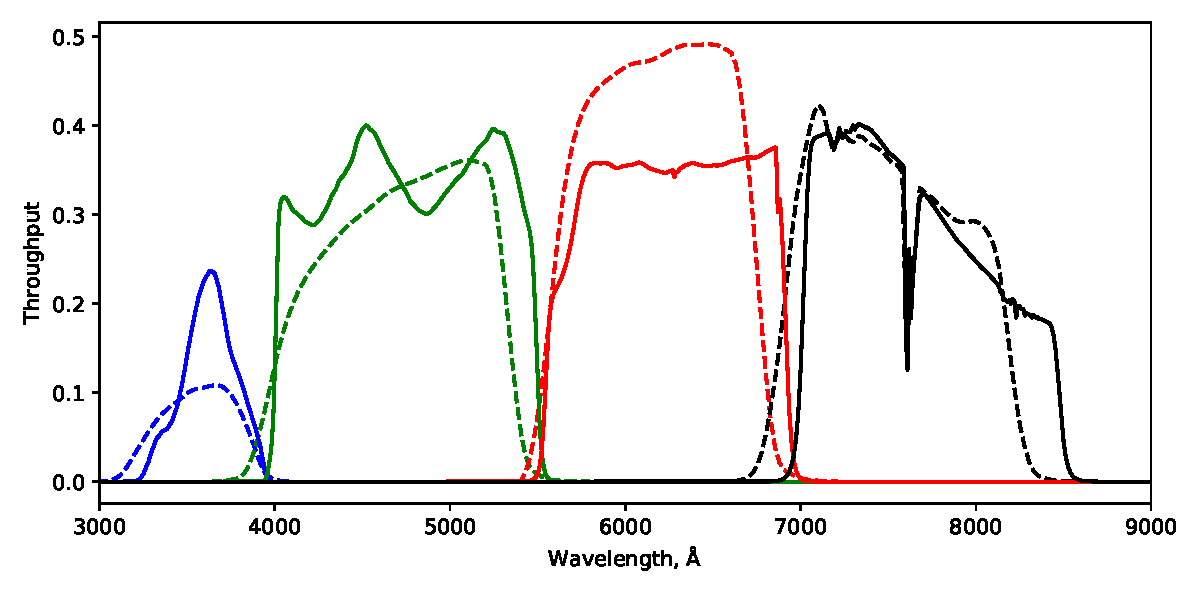
\includegraphics[width=\columnwidth]{figures/three_cvs_with_weird_colours/GeneralFigs/bandpass_diffs_SDSS_dots_UCAMNTT_solid.pdf}
    \caption{The differences in photometric throughput for SDSS filter system ({\bf dotted lines}), and ULTRACAM Super SDSS filters, for ULTRACAM mounted on the NTT ({\bf solid lines}). Blue: $u$ bands, Green: $g$ bands, Red: $r$ bands, Black: $i$ bands. Both throughputs include atmospheric extinction of $\chi = 1.3$.}
    \label{fig:sdss vs super filters}
\end{figure}

To perform the colour corrections, the following equation for the magnitude of a star was used, using the $g'$\ band as an example:
\begin{equation}
    \label{eqn:gen magnitudes}
    g' = g_{\rm inst} + \chi k_{\rm ext} + g_{\rm zp} + c_{\rm g, sup}(g'-r')
\end{equation}
where $g_{\rm zp}$\ is the zero point, $g_{\rm inst} = -2.5 \rm log(ADU_{\rm exp}/{\it t}_{\rm exp})$
for an exposure time of $t_{\rm exp}$, and $c_{\rm g, sup}$\ is the colour term correction gradient. In theory, the atmospheric extinction term also has some colour dependency, as extinction varies with wavelength. However, the effect is negligible between these photometric systems, so it is omitted.

The optical path of each system was simulated using the \texttt{pysynphot} package, with measured throughputs of all ULTRACAM and HiPERCAM components in the optical path. Precomputed stellar models from \citet{Dotter2016} and \citet{Choi2016} were used to generate the \teff\ and \logg\ values of an $8.5$\ Gyr isochrone for main sequence stars with masses from 0.1 to 3 $M_\odot$, spanning from \logg $= 3.73 \to 5.17$, and $\rm{T_{eff}} = 2900K \to 10,300K$. The Phoenix model atmospheres \citep{allard2012} were used to generate model spectra of each mass, which was then folded through each optical path to calculate an AB magnitude. In addition, white dwarf models with \logg$=8.5$\ were similarly processed \citep{koester2010, tremblay2009}, to asses the impact of the different spectral shape on the resulting colour terms.

The colour terms between the SDSS and Super SDSS systems were then synthesised, e.g., $g'-g_{\rm sup}$, on ULTRACAM and HiPERCAM for each model atmosphere. These data were plotted against synthesised SDSS colours, i.e. $(u'-g')$, $(g'-r')$, $(g'-i')$, and a straight line was fit to the colour relationship. In the example case of $g'-g_{\rm sup}$, this would be
\begin{align*}
    % g' &= g_{\rm sup} + g_{\rm zp} + c_{\rm g, sup}(g'-r') \\
    g' - g_{\rm sup} &= g_{\rm zp} + c_{\rm g, sup}(g'-r')
\end{align*}
These relationships are shown for HiPERCAM in Figure~\ref{fig:observations:ULTRACAM colour corrections} for all four Super SDSS filters used to observe these CVs, and Table~\ref{table:observations:all ULTRACAM colour corrections} and Table~\ref{table:observations:all HiPERCAM colour corrections} contain the coefficients of each colour term correction for both HiPERCAM and ULTRACAM.
$(u'-g')$\ was used to correct $u$\ magnitudes, $(g'-r')$\ was used to correct $g$\ and $r$\ magnitudes, $(g'-i')$\ was used to correct the $i$\ band.
These colour corrections are not generally the same for main sequence stars and white dwarfs, though the colours of the white dwarfs presented in this work are all such that the discrepancy is on the order of a few percent, and is considered negligible.

\noindent\begin{minipage}{\linewidth}
    \centering

    \captionof{table}{ULTRACAM colour term best fit lines from Figure~\ref{fig:observations:ULTRACAM colour corrections}. The data are modelled by equations of the form $(u'-u_{\rm sup}) = \phi + c_u(u'-g')$, with $c_u$\ being the relevant colour gradient.}
    \label{table:observations:all ULTRACAM colour corrections}
    \begin{tabular}{cccc}
        Correction          & Diagnostic    & $\phi$    & $c$ \\
        \hline
        \hline
        $(u'-u_{\rm sup})$  &  $(u'-g')$    & 0.003     & 0.036 \\
                            &  $(g'-r')$    & 0.033     & 0.063 \\
                            &  $(g'-i')$    & 0.038     & 0.044 \\
        \hline
        $(g'-g_{\rm sup})$  &  $(u'-g')$    & -0.001    & 0.014 \\
                            &  $(g'-r')$    & 0.010     & 0.027 \\
                            &  $(g'-i')$    & 0.012     & 0.018 \\
        \hline
        $(r'-r_{\rm sup})$  &  $(u'-g')$    & -0.017    & 0.016 \\
                            &  $(g'-r')$    & -0.004    & 0.032 \\
                            &  $(g'-i')$    & -0.002    & 0.022 \\
        \hline
        $(i'-i_{\rm sup})$  &  $(u'-g')$    & -0.031    & 0.020 \\
                            &  $(g'-r')$    & -0.015    & 0.040 \\
                            &  $(g'-i')$    & -0.012    & 0.028 \\
        \hline
        \hline
    \end{tabular}

    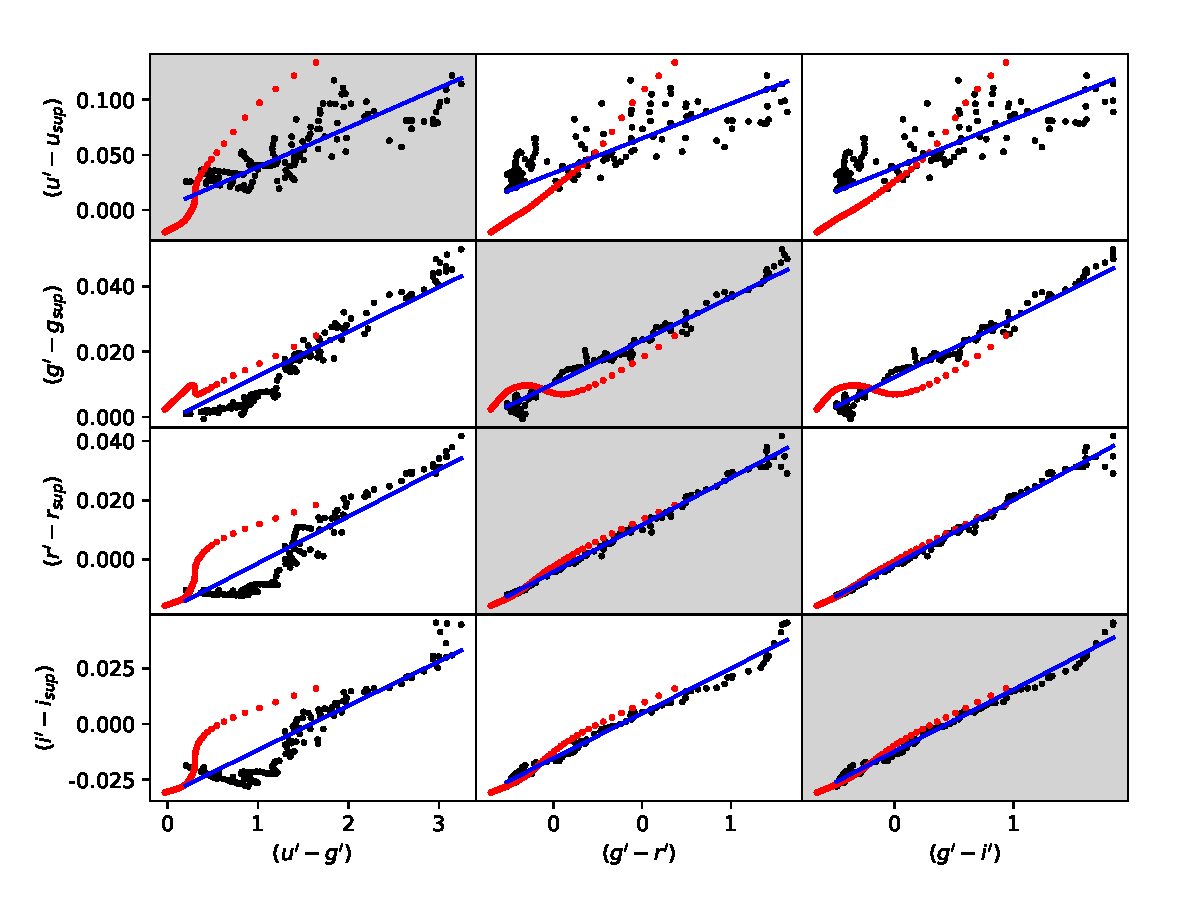
\includegraphics[width=\textwidth]{figures/observations/colour_term_tracks_UCAM.pdf}
    \captionof{figure}{The difference between the classic SDSS photometric system, and the ULTRACAM SuperSDSS filters on the NTT, as a function of SDSS colours, are calculated for model atmospheres. {\bf Red points} are Koester white dwarf models, {\bf black points} are Phoenix main sequence model atmospheres, and the {\bf blue line} is the best fit straight line to both datasets. When applying colour corrections, the highlighted relations were used.}
    \label{fig:observations:ULTRACAM colour corrections}
\end{minipage}

\noindent\begin{minipage}{\linewidth}
    \centering

    \captionof{table}{HiPERCAM colour term best fit lines from Figure~\ref{fig:observations:HiPERCAM colour corrections}. The data are modelled by equations of the form $(u'-u_{\rm sup}) = \phi + c_u(u'-g')$, with $c_u$\ being the relevant colour gradient.}
    \label{table:observations:all HiPERCAM colour corrections}
    \begin{tabular}{cccc}
            Correction          & Diagnostic & $\phi$   & $c$ \\
            \hline
            \hline
            $u'-u_{\rm sup}$    & $(u'-g')$   &   0.096   & 0.054\\
                                & $(g'-r')$   &   0.150   & 0.029\\
                                & $(g'-i')$   &   0.152   & 0.022\\
            \hline
            $g'-g_{\rm sup}$    & $(u'-g')$   &   0.008   & 0.023\\
                                & $(g'-r')$   &   0.010   & 0.045\\
                                & $(g'-i')$   &   0.014   & 0.031\\
            \hline
            $r'-r_{\rm sup}$    & $(u'-g')$   &   0.000   & 0.001\\
                                & $(g'-r')$   &   0.001   & 0.003\\
                                & $(g'-i')$   &   0.001   & 0.002\\
            \hline
            $i'-i_{\rm sup}$    & $(u'-g')$   &   0.033   & 0.022\\
                                & $(g'-r')$   &   0.016   & 0.044\\
                                & $(g'-i')$   &   0.012   & 0.030\\
            \hline
            \hline
    \end{tabular}

    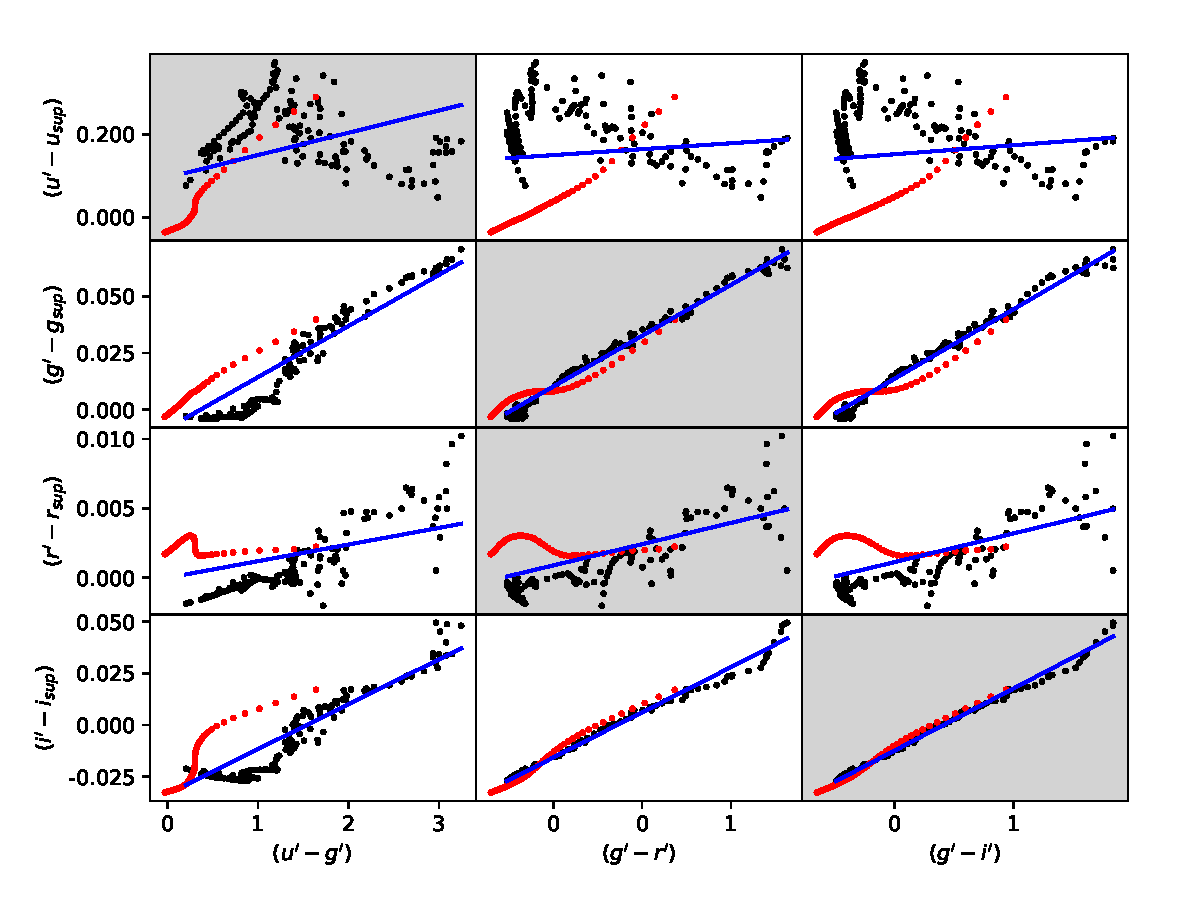
\includegraphics[width=\textwidth]{figures/observations/colour_term_tracks_HCAM.pdf}
    \captionof{figure}{As Figure~\ref{fig:observations:ULTRACAM colour corrections}}
    \label{fig:observations:HiPERCAM colour corrections}
\end{minipage}


\subsection{Calculating comparison star magnitudes}
\label{sect:comparison star mag calc}

The stars in the target frame often do not have known brightnesses in the SDSS photometric system, and so this must be determined by observation. The network of SDSS photometric standards provided by \citet{smith2002} are used as calibrating objects, with robust, accurate known magnitudes. By observing a flux standard during clear conditions, the comparison stars' magnitude can then be calculated from a similarly clear observation.
Equation \ref{eqn:gen magnitudes} was used to calculate the zero points of the telescope/instrument combination in each band from a standard star observation.

The comparison star magnitudes were then calculated from observations.
Since the colour term corrections are dependent on SDSS colours, an iterative approach was used to converge on these values.
SDSS magnitudes are related to the instrumental magnitudes by:
\begin{align*}
    u' =& u_{\rm inst,0} + u_{\rm zp} + c_{\rm u, sup}(u' - g') \\
    g' =& g_{\rm inst,0} + g_{\rm zp} + c_{\rm g, sup}(g' - r') \\
    r' =& r_{\rm inst,0} + r_{\rm zp} + c_{\rm r, sup}(g' - r') \\
    i' =& i_{\rm inst,0} + i_{\rm zp} + c_{\rm i, sup}(g' - i') \\
\end{align*}
Initially, $u',g',r',i'$\ magnitudes are set equal to the instrumental magnitudes, and a new set of $u',g',r',i'$\ magnitudes are calculated. The new values are then used to repeat the calculation until a new iteration produces no change, typically after $\sim$4 loops.


\subsection{Producing a flux-calibrated target lightcurve}
\label{sect:flux calibrating the lightcurve}

Finally, the target lightcurves can be calculated. Broadly, this encompasses two processes: the target star lightcurve must be corrected for transparency variations, and then converted from ADU counts to calibrated flux.
As the aim is to produce a flux-calibrated lightcurve in the SDSS photometric system, from observations using a significantly different photometric system, the simple ADU ratio between the target and comparison is insufficient.
Consider the target star $g'$ magnitude and flux, $g^t, F^t$, and comparison star $g'$ magnitude and flux, $g^c, F^c$:
\begin{align*}
    g^t =& g^t_{\rm inst,0} + g_{\rm zp} + c_{\rm g, sup}(g'-r')^t \\
    g^c =& g^c_{\rm inst,0} + g_{\rm zp} + c_{\rm g, sup}(g'-r')^c \\
\end{align*}
since,
\begin{equation*}
    g^t - g^c = -2.5{\rm log}\Big(\frac{F^t}{F^c}\Big) \\
\end{equation*}
we can write
\begin{align*}
    % g^t - g^c =& g^t_{\rm inst,0} - g^c_{\rm inst,0} + c_{\rm g, sup}\big((g-r)^t - (g-r)^c\big) \\
    \frac{F^t}{F^c} =& 10^{-0.4(g^t_{\rm inst,0} - g^c_{\rm inst,0})} \cdot 10^{-0.4c_{\rm g, sup}\big((g'-r')^t - (g'-r')^c\big)} \\
    % \frac{F^t}{F^c} =& \frac{ADU^t/s}{ADU^c/s}\cdot 10^{c_{\rm g, sup}\big((g-r)^t - (g-r)^c\big)} \\
    \frac{F^t}{F^c} =& \frac{ADU^t}{ADU^c}\cdot K^{t,c} \\
\end{align*}
where $K^{t,c} = 10^{-0.4c_{\rm g, sup}\big((g'-r')^t - (g'-r')^c\big)}$.
This accounts for differences in wavelength response between the two systems when calculating the flux ratio, and is applied to each frame. The $(g'-r')^t$\ magnitudes are calculated using a sigma-clipped mean instrumental magnitudes computed from all frames in the observation. In practice, the factor $K^{t,c}$\ varies from $\sim 1.0 - 1.1$\ for our observations.

While developing this correction method, some verification tests were performed.
ASASSN-16kr was observed in both the standard SDSS filters in 2018, and the super SDSS filters in 2019. This presented an opportunity to compare the corrected 2019 data with the fluxes observed in 2018. Additionally, both ASASSN-16kr and SSSJ0522-3505 use multiple standard stars across observations, which should agree if the calibration has been done correctly. In all cases, the flux-calibrated lightcurves were similar and the white dwarf colours consistent, suggesting that this method of flux calibration is indeed accurate.

We add a 3\% systematic error in quadrature to the white dwarf fluxes when fitting for the effective temperature. This is a practice established by \citet{McAllister2019}, to account for possible systematic error in flux calibration and modelling.

\newpage
\section{Catalogue of observations}

\todo{Make a Table of observations.}The observations analysed in this work span the full decade from 2011, through to 2021, and have been taken from multiple sites as the instruments move from telescope to telescope. To aid with the readability, a key is provided in Table~\ref{tab:observation acronyms} of the acronyms used for instruments and telescopes.

\begin{table}
    \centering
    \begin{tabular}{c|c}
        Acronym & Expansion \\
        \hline
        NTT & New Technology Telescope \\
        GTC & Gran Telescopio Canarias \\
        TNT & Thai National Telescope \\
        WHT & William Herschel Telescope \\
        VLT & Very Large Telescope \\
        HCAM & HiPERCAM \\
        UCAM & ULTRACAM \\
        USPEC & ULTRASPEC \\
    \end{tabular}
    \caption{Acronyms used in the observation summaries.}
    \label{tab:observation acronyms}
\end{table}
